%!TEX root = ../../Compte-rendu.tex

\begin{figure}[H]
	\begin{center}
		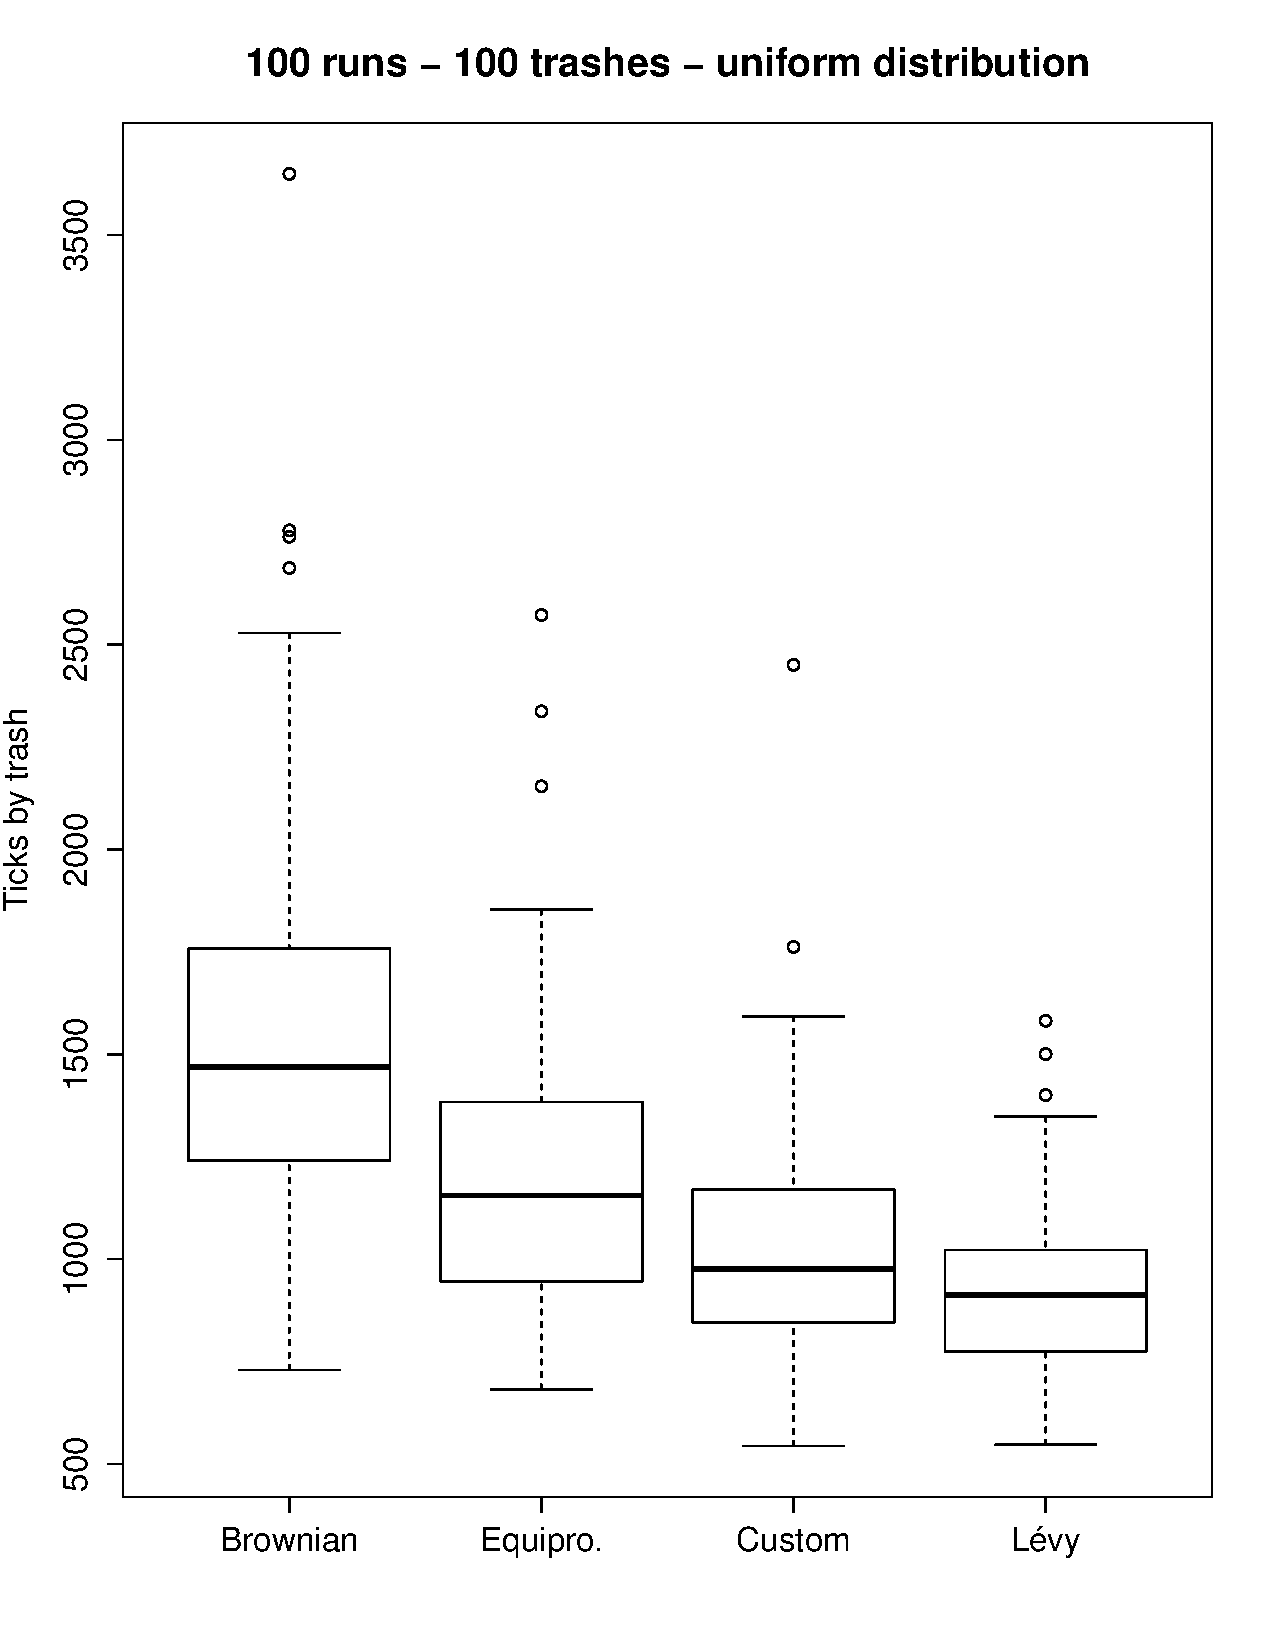
\includegraphics[height=10cm]{diagrams/100TrRnd_all.pdf}
		\caption{Résultat des mesures pour 100 débris uniformément répartis}
		\label{fig:100Trashes_Rnd}
	\end{center}
\end{figure}
Nous avons pour les différentes stratégies les statistiques suivantes :
\begin{figure}[H]
	\begin{center}
		\begin{tabular}{| c || c | c | c | c | }
			\hline
			&Brown.&Equi.&Custom&Lévy \\
			\hline
			\hline
			md&1469&1155&975&912\\
			mean&1551&1197&1036&925\\
			min & 729 & 682 & 543 & 546 \\
			max & 3650 & 2573 & 2451 & 1582 \\
			sd&490&331&296&208\\
			p-val&$\ll 5\%$&$\ll 5\%$&$\ll 5\%$&$\ll 5\%$\\
			\hline
		\end{tabular}
		\caption{Statistiques pour 100 débris distribués uniformément}
	\end{center}
\end{figure}

En partant de la stratégie Brownian et en allant à celle de Lévy
en passant par Equiprobable et Custom, nous pouvons constater
que nous avons de meilleurs résultats, que ce soit pour leur médiane
comme pour leur fiabilité ainsi que leur valeur minimale et maximale.
